%%% DOCUMENT TYPE %%%%%%%%%%%%%%%%%%%%%%%%%%%%%%%%%%%%%%%%%%%%%%%%%%%%%%%%%%%%%%



%%% SETUP %%%%%%%%%%%%%%%%%%%%%%%%%%%%%%%%%%%%%%%%%%%%%%%%%%%%%%%%%%%%%%%%%%%%%%

%%% DOCUMENT TYPE %%%%%%%%%%%%%%%%%%%%%%%%%%%%%%%%%%%%%%%%%%%%%%%%%%%%%%%%%%%%%%

\documentclass[9pt, a4paper, twocolumn, landscape]{extarticle}

%%% PACKAGES %%%%%%%%%%%%%%%%%%%%%%%%%%%%%%%%%%%%%%%%%%%%%%%%%%%%%%%%%%%%%%%%%%%

% Encoding

\usepackage[utf8]{inputenc}
\usepackage[T1]{fontenc}

% Geometry

\usepackage{geometry} % edit margins of paper
\usepackage{setspace} % edit line spacing
\usepackage{fancyhdr} % header, footer
\usepackage{titlesec} % edit format of titles

% Visual

\usepackage[dvipsnames]{xcolor} % colors
\usepackage{tikz} % graphics
\usepackage[framemethod=tikz]{mdframed} % frames, better theorems

% Math

\usepackage{amsmath} % math tools
\usepackage{amssymb} % math symbols
\usepackage{amsthm} % thereoms
\usepackage{mathtools} % math tools

% Referencing

\usepackage{nameref}
\usepackage{hyperref}
\usepackage{cleveref}

% Useful

\usepackage[shortlabels]{enumitem} % enumerations

% Other

\usepackage{lastpage} % get number of last page
\usepackage{physics}
\usepackage{bbm}

%%% MARGINS %%%%%%%%%%%%%%%%%%%%%%%%%%%%%%%%%%%%%%%%%%%%%%%%%%%%%%%%%%%%%%%%%%%%

\geometry{a4paper, landscape, left=10mm, right=10mm, top=10mm, bottom=10mm, includehead}

%%% COLORS %%%%%%%%%%%%%%%%%%%%%%%%%%%%%%%%%%%%%%%%%%%%%%%%%%%%%%%%%%%%%%%%%%%%%

%%% TITLES %%%%%%%%%%%%%%%%%%%%%%%%%%%%%%%%%%%%%%%%%%%%%%%%%%%%%%%%%%%%%%%%%%%%%

\colorlet{color-section}                {Blue}
\colorlet{color-subsection}             {RoyalPurple}
\colorlet{color-paragraph}             {MidnightBlue}
\colorlet{color-subsubsection}	{CadetBlue}
%%% MATH BOXES %%%%%%%%%%%%%%%%%%%%%%%%%%%%%%%%%%%%%%%%%%%%%%%%%%%%%%%%%%%%%%%%%

\colorlet{color-definition}              {Blue!20}%{SpringGreen!20}
\colorlet{color-theorem}                {Brown!25}%{Apricot!13}
\colorlet{color-proposition}            {ProcessBlue!13}% {Apricot!13}
\colorlet{color-corollary}              {Salmon!12}%{Apricot!13}
\colorlet{color-lemma}                  {Brown!7}%{Apricot!13}
\colorlet{color-remark}                 {Gray!4}
\colorlet{color-example}                {Lavender!7}
% \colorlet{color-proof}                  {FILL COLOR HERE}


%%% CAPTIONS %%%%%%%%%%%%%%%%%%%%%%%%%%%%%%%%%%%%%%%%%%%%%%%%%%%%%%%%%%%%%%%%%%%

%%% CAPTION DEFINITION %%%%%%%%%%%%%%%%%%%%%%%%%%%%%%%%%%%%%%%%%%%%%%%%%%%%%%%%%

\newcommand*{\definitionname}{Definition}
\newcommand*{\theoremname}{Theorem}
\newcommand*{\propositionname}{Proposition}
\newcommand*{\corollaryname}{Corollary}
\newcommand*{\lemmaname}{Lemma}
\newcommand*{\remarkname}{Remark}
\newcommand*{\examplename}{Example}


%%% SHORTCUTS %%%%%%%%%%%%%%%%%%%%%%%%%%%%%%%%%%%%%%%%%%%%%%%%%%%%%%%%%%%%%%%%%%

%%% SINGLE SYMBOLS %%%%%%%%%%%%%%%%%%%%%%%%%%%%%%%%%%%%%%%%%%%%%%%%%%%%%%%%%%%%

% Logic

% \forall exists
% \exists exists
% \lnot exists
% \lor exists
% \land exists
\newcommand*{\limp}{\rightarrow}
\newcommand*{\limps}{\; \limp \;} % \limp with some space around
\newcommand*{\leqv}{\leftrightarrow}
\newcommand*{\leqvs}{\; \leqvs \;} % \leqv with some space around

% Meta Logic

% \implies exists
% \iff exists

% Colon Stuff

\newcommand*{\cl}{\colon}
\newcommand*{\cleq}{\coloneqq}
\newcommand*{\eqcl}{\eqqcolon}

% Sets

\newcommand*{\N}{\mathbb{N}} % natural numbers
\newcommand*{\Z}{\mathbb{Z}} % integers
\newcommand*{\Q}{\mathbb{Q}} % rational numbers
\newcommand*{\R}{\mathbb{R}} % real numbers
\newcommand*{\C}{\mathbb{C}} % complex numbers

%%% MATH OPERATORS %%%%%%%%%%%%%%%%%%%%%%%%%%%%%%%%%%%%%%%%%%%%%%%%%%%%%%%%%%%%%

% General

\DeclareMathOperator{\id}{id}
\DeclareMathOperator{\sgn}{sgn}
\DeclareMathOperator{\vol}{vol}
\DeclareMathOperator{\supp}{supp}
\let\grad\relax
\DeclareMathOperator{\grad}{grad}
\DeclareMathOperator{\rot}{rot}
\let\div\relax
\DeclareMathOperator{\div}{div}
%%% TEMPLATES %%%%%%%%%%%%%%%%%%%%%%%%%%%%%%%%%%%%%%%%%%%%%%%%%%%%%%%%%%%%%%%%%%

% General

% write a set definition like: { #1 | #2 }
\newcommand*{\setdefinition}[2]{
  \{#1 \mid #2\}
}

% write a nice map definition
\newcommand*{\mapdefinition}[5]{
  \begin{align*}
    #1 \cl #2 &\to     #3 \\
           #4 &\mapsto #5
  \end{align*}
}


%%% FORMATTING %%%%%%%%%%%%%%%%%%%%%%%%%%%%%%%%%%%%%%%%%%%%%%%%%%%%%%%%%%%%%%%%%

%%% HEADER, FOOTER %%%%%%%%%%%%%%%%%%%%%%%%%%%%%%%%%%%%%%%%%%%%%%%%%%%%%%%%%%%%%

\pagestyle{fancy}
\fancyhf{} % clear everything
\lhead{}
\chead{\bfseries Quantum Physics}
\rhead{Seite \thepage / \pageref*{LastPage}}
\lfoot{}
\cfoot{}
\rfoot{}

%%% TITLE FORMAT %%%%%%%%%%%%%%%%%%%%%%%%%%%%%%%%%%%%%%%%%%%%%%%%%%%%%%%%%%%%%%%

\setcounter{secnumdepth}{2}

\titleformat{\chapter}[display]
{\normalfont\huge\bfseries}{\chaptertitlename\ \thechapter}{20pt}{\Huge}
\titleformat{\section}[frame]
{\normalfont\LARGE\bfseries\color{color-section}\scshape\filright}{\thesection}{1ex}{\filcenter}
\titleformat{\subsection}
{\normalfont\large\bfseries\color{color-subsection}}{\thesubsection}{1em}{}
\titleformat{\subsubsection}
{\normalfont\normalsize\bfseries\color{color-subsubsection}}{\thesubsubsection}{1em}{}
\titleformat{\paragraph}[runin]
{\normalfont\normalsize\bfseries\color{color-paragraph}}{\theparagraph}{1em}{}
\titleformat{\subparagraph}[runin]
{\normalfont\normalsize\bfseries}{\thesubparagraph}{1em}{}

%%% SPACING %%%%%%%%%%%%%%%%%%%%%%%%%%%%%%%%%%%%%%%%%%%%%%%%%%%%%%%%%%%%%%

% Titles

\titlespacing*{\chapter}{0pt}{50pt}{40pt}
\titlespacing*{\section}{0pt}{3.5ex plus 1ex minus .2ex}{2.3ex plus .2ex}
\titlespacing*{\subsection}{0pt}{3.25ex plus 1ex minus .2ex}{1.5ex plus .2ex}
\titlespacing*{\subsubsection}{0pt}{3.25ex plus 1ex minus .2ex}{1.5ex plus .2ex}
\titlespacing*{\paragraph}{0pt}{1.25ex plus 1ex minus .2ex}{1em}
\titlespacing*{\subparagraph}{\parindent}{3.25ex plus 1ex minus .2ex}{1em}

% Text, Paragraphs

%\setstretch{1.05} % scaling of space between lines
%\setlength{\parindent}{0pt} % indentation of paragraphs
%\setlength{\parskip}{4.0pt plus 1.0pt minus 1.0pt} % space between paragraphs
\setlength{\parskip}{0pt}

%%% SYMBOLS USED BY NUMBERINGS, ENVIRONMENTS, ... %%%%%%%%%%%%%%%%%%%%%%%%%%%%%%

% \renewcommand*\qedsymbol{$\blacksquare$} % alternative QED symbol
\renewcommand{\thefootnote}{\arabic{footnote}} % normal footnotes on page
\renewcommand{\thempfootnote}{\fnsymbol{mpfootnote}} % footnotes on minipages, e.g. in mdframed environments

%%% LISTS, ENUMERATIONS %%%%%%%%%%%%%%%%%%%%%%%%%%%%%%%%%%%%%%%%%%%%%%%%%%%%%%%%

% 'itemize'

\setlist[itemize]{noitemsep, topsep=0pt}

% 'enumerate'

% no special settings at the moment

% 'description'

% no special settings at the moment

% 'axioms'

\newlist{axioms}{enumerate}{2}
\setlist[axioms]{itemsep=0pt,label*=\arabic*.}

%%% MDFRAMED PATCH %%%%%%%%%%%%%%%%%%%%%%%%%%%%%%%%%%%%%%%%%%%%%%%%%%%%%%%%%%%%%

\usepackage{xpatch}

\makeatletter
\xpatchcmd{\endmdframed}
  {\aftergroup\endmdf@trivlist\color@endgroup}
  {\endmdf@trivlist\color@endgroup\@doendpe}
  {}{}
\makeatother

%%% MDFRAMED STYLES %%%%%%%%%%%%%%%%%%%%%%%%%%%%%%%%%%%%%%%%%%%%%%%%%%%%%%%%%%%%

% thick frame and bar for title

\mdfdefinestyle{style-box}{
  skipabove=1.5ex plus .5ex minus .2ex,
  skipbelow=1ex plus .2ex minus .2ex,
  linewidth=2pt,
  linecolor=Gray!20,
%   roundcorner=3pt,
  innerleftmargin=0.5\baselineskip,
  innerrightmargin=0.5\baselineskip,
  innertopmargin=0.4\baselineskip,
  innerbottommargin=0.4\baselineskip,
  frametitlebackgroundcolor=Gray!20,
  frametitleaboveskip=0.3pt,
  frametitlebelowskip=0.3pt,
  theoremseparator=,
  theoremspace=\hfill,
  theoremtitlefont=\mdseries\scshape,
  nobreak=true
}

% highlighted background

\mdfdefinestyle{style-background}{
  skipabove=1.5ex plus .5ex minus .2ex,
  skipbelow=1ex plus .2ex minus .2ex,
  hidealllines=true,
  backgroundcolor=Gray!5,
  innerleftmargin=0.5\baselineskip,
  innerrightmargin=0.5\baselineskip,
  innertopmargin=0.4\baselineskip,
  innerbottommargin=0.4\baselineskip,
}

% thin frame

\mdfdefinestyle{style-leftline}{
  skipabove=1.5ex plus .5ex minus .2ex,
  skipbelow=1ex plus .2ex minus .2ex,
  linewidth=1pt,
  linecolor=Gray!50,
  topline=false,
  bottomline=false,
  rightline=false,
  innerleftmargin=0.5\baselineskip,
  innerrightmargin=0,
  innertopmargin=0.2\baselineskip,
  innerbottommargin=0.0\baselineskip,
}

%%% ENVIRONMENTS %%%%%%%%%%%%%%%%%%%%%%%%%%%%%%%%%%%%%%%%%%%%%%%%%%%%%%%%%%%%%%%

% Definition

\mdtheorem[
  style=style-box,
  linecolor=color-definition,
  frametitlebackgroundcolor=color-definition
]{definition}{\definitionname}[section]

% Theorem

\mdtheorem[
  style=style-box,
  linecolor=color-theorem,
  frametitlebackgroundcolor=color-theorem,
  font=\itshape
]{theorem}{\theoremname}[section]

% Proposition

\mdtheorem[
  style=style-box,
  linecolor=color-proposition,
  frametitlebackgroundcolor=color-proposition,
  font=\itshape
]{proposition}[theorem]{\propositionname}

% Corollary

\mdtheorem[
  style=style-box,
  linecolor=color-corollary,
  frametitlebackgroundcolor=color-corollary,
  font=\itshape
]{corollary}[theorem]{\corollaryname}

% Lemma

\mdtheorem[
  style=style-box,
  linecolor=color-lemma,
  frametitlebackgroundcolor=color-lemma,
  font=\itshape
]{lemma}[theorem]{\lemmaname}

\theoremstyle{remark}

% Remark

\newtheorem*{remark}{\remarkname}
\surroundwithmdframed[
  style=style-background,
  backgroundcolor=color-remark
]{remark}

% Example

\newtheorem*{example}{\examplename}
\surroundwithmdframed[
  style=style-background,
  backgroundcolor=color-example
]{example}

% Proof

\surroundwithmdframed[
  style=style-leftline
]{proof}

%%% TEXT FORMATTING %%%%%%%%%%%%%%%%%%%%%%%%%%%%%%%%%%%%%%%%%%%%%%%%%%%%%%%%%%%%

% definitions
\let\epsilon\varepsilon
\renewcommand\emptyset{\varnothing}
\newcommand*{\df}[1]{\colorbox{color-definition}{\emph{#1}}}


%%% LANGUAGE %%%%%%%%%%%%%%%%%%%%%%%%%%%%%%%%%%%%%%%%%%%%%%%%%%%%%%%%%%%%%%%%%%%

%%% SETUP %%%%%%%%%%%%%%%%%%%%%%%%%%%%%%%%%%%%%%%%%%%%%%%%%%%%%%%%%%%%%%%%%%%%%%

\usepackage[english]{babel}

%%% CAPTION REDEFINITION %%%%%%%%%%%%%%%%%%%%%%%%%%%%%%%%%%%%%%%%%%%%%%%%%%%%%%%



%%% HYPHENATION %%%%%%%%%%%%%%%%%%%%%%%%%%%%%%%%%%%%%%%%%%%%%%%%%%%%%%%%%%%%%%%%


\usepackage[arrow, matrix, curve]{xy}
\usepackage{wrapfig}
\usepackage{bm}
\usepackage{multicol}
\usepackage{xcolor}
\usepackage{mathrsfs} 
\renewcommand\vec{\boldsymbol}

%%% DOCUMENT %%%%%%%%%%%%%%%%%%%%%%%%%%%%%%%%%%%%%%%%%%%%%%%%%%%%%%%%%%%%%%%%%%%

\begin{document}

\section{Stuff dump}

\paragraph{Cambell Baker Hausdorf} Für alle $t \in \mathbb{R}$ 
$$ 
\exp(t A) \exp(t B)= \exp \left(t A+t B+\frac{t^2}{2}[A, B]
+\frac{t^3}{12} [A,[A, B]] +\frac{t^3}{12}[B,[B, A]]+\mathscr{O}\left(t^4\right)\right)
$$
 


\paragraph{Bernoulli Trial} Probability of $k$ successes in a bernoulli experiment $B(n,p)$:
$$P(k)=\left(\begin{array}{l}
  n \\
  k
  \end{array}\right) p^k q^{n-k} $$

\paragraph{Bayes' rule}  $$
\operatorname{Pr}[A \mid B \wedge C]=\frac{\operatorname{Pr}[B \mid A \wedge C]}{\operatorname{Pr}[B \mid C]} \operatorname{Pr}[A \mid C]
$$

\paragraph{Maxwell equations} we have \\
$ \nabla E = \frac{\rho}{\epsilon_0}  \quad  $  \ (Gauss law)   \\
$ \nabla B = 0 $ \\
$ \nabla \times E = \ - \frac{\partial B}{\partial t} \quad  $ \  (Faraday's law of induction) \\
$ \nabla \times B = \frac{1}{c^2} \frac{ \partial E}{\partial t} + \mu_0 J + \epsilon_0 \frac{\partial P} {\partial t} \quad $ \ (Ampere's law)


\paragraph{Bloch sphere}$\hat{n}(\theta, \phi)$ on Bloch sphere with $\theta \in (0, \pi)$, $\phi \in (0,2 \pi)$. 
For $- \hat{n}$ we have $(\theta, \phi) \to (\pi - \theta , \phi + \pi) $.\\
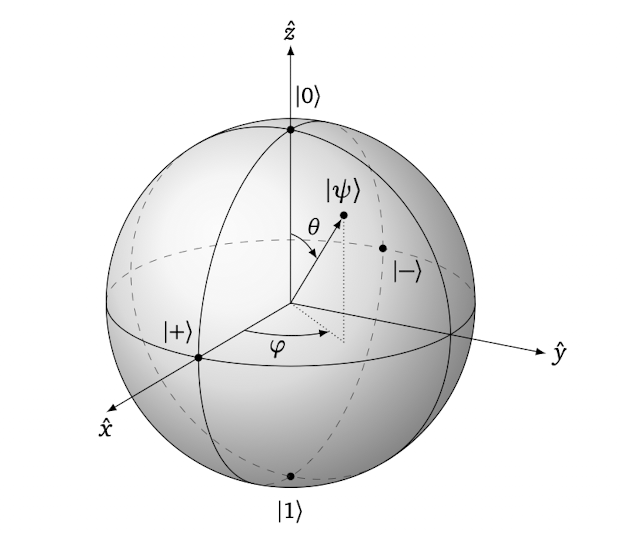
\includegraphics[scale=0.2]{fig/BlochSph.png}

\paragraph{Monte Carlo Methods} Class of algorithms that rely on random sampling to obtain numerical results

\paragraph{Delta distribution}
\begin{itemize}
  \item $\int d x e^{i k \cdot x}=(2 \pi) \delta(k)$
  \item $\int_{-\infty}^{+\infty} d x \delta(g(x))=\sum_i \frac{1}{\left|g^{\prime}\left(x_i\right)\right|} $
\end{itemize}

%%%%%%%%%%%%%%%%%%%%%%%%%%%%%%%%%%%%%%%%%%%%%%%%%%%%%%%%%%%%%%%%%%%%%%%%%%%%%%% QIT
\section{Quantum Information Theory}
\paragraph{Quantum probability}
$Pr[|\Lambda] = \Trace{\Lambda \rho} $\\
probabity density: $\quad \rho \in \operatorname{Lin}(\mathcal{H}), \quad \rho \geq 0, \quad \Trace[p] =1$\\
effect / measuremnt: $\Lambda \in \operatorname{Lin}(\mathcal{H}), \quad \Lambda \geq 0, \quad \Lambda \leq \mathbb{1}$\\

positivity of operators: $S \geq 0$ if $\langle v|S| v\rangle \geq 0 \text { for all } v \in \mathcal{H}$

\paragraph{POVM: postive operator valued measure} set of effects $\{ \Lambda (x)\}^n_{x=1}$ such that
$\Lambda(x) \in \operatorname{Lin}(\mathcal{H}) : \Lambda(x) \geq 0 \ \forall x, \ \sum_x \Lambda(x) =$ $1$

\paragraph{Trace (abstract)} $\Trace{\ketbra*{\Phi}{\Psi}} := \braket*{\Psi}{\Phi}$, then extend linearly. Then we have further\\
$\Trace[ABC]= \Trace[CAB]$ and for basis transformations we habe $\Tr[U \rho U^* ]= \Tr[\rho]$\\

\subsection{Composite Systems} 
$\mathcal{H}_{AB} = \mathcal{H}_A \otimes \mathcal{H}_B$\\
$\ket{+}_A\otimes \ket{+}_B = \ket*{++}_{AB} = \frac{1}{2} (\ket*{00}_{AB}+ \ket*{01}_{AB}+ \ket*{10}_{AB}+\ket*{11}_{AB})$\\
product state: $\ket{\Psi}\otimes \ket*{\phi} = \ket*{\Psi}_{AB} \quad$ entagled state: $\ket*{\Psi}_{AB}$ such that it cannot be written as productstate.\\
Partial trace $\Tr_{AB}[M_{AB}] = \Tr_A[\Tr_B[M_{AB}]]$

\paragraph{Technical stuff}
\begin{itemize}
  \item Pauli Operators: $\sigma_1=\left(\begin{array}{cc}
    0 & 1 \\
    1 & 0
    \end{array}\right), \quad \sigma_2=\left(\begin{array}{cc}
    0 & -\mathrm{i} \\
    \mathrm{i} & 0
    \end{array}\right), \quad \sigma_3=\left(\begin{array}{cc}
    1 & 0 \\
    0 & -1
    \end{array}\right)$
  \item $\left[\sigma_i, \sigma_j\right]=2 i \varepsilon_{i j k} \sigma_k$
  \item porbability density is pure state iff: $\Tr[p^2]=1$
  \item positivity of operators: $S \geq 0$ if $\langle v|S| v\rangle \geq 0 \text { for all } v \in \mathcal{H}. \quad $ $\longrightarrow \quad$ $S$ is hermitian


\end{itemize}


%%%%%%%%%%%%%%%%%%%%%%%%%%%%%%%%%%%%%%%%%%%%%%%%%%%%%%%%%%%%%%%%%%%%%%%%%%%%%%% QFT
\section{Quantum Field Theory I}

\paragraph{Basis transformation} $\{ \ket*{i} \to \ket*{\lambda} \}$  for orthonormal Basis:\\ 
$\ket*{\lambda } = \sum_i \ket*{i} \ketbra*{i}{\lambda} \quad   \implies  \quad $ if $\hat{a}_i^\dagger \ket*{0} = \ket*{i}$ then 
$\hat{a}_\lambda^\dagger \ket*{0} = \sum_i \ketbra*{i}{\lambda} \hat{a}_i^\dagger \ket{0} = \ket*{\lambda} $\\

Like this any Hamitonian of the form $H=T+U+V$ (e.g.) \\ 
$H=\sum_{i=1}^N \frac{\mathbf{p}_i^2}{2 m}-\sum_{i=1}^N \frac{Z e^2}{\left|\mathbf{x}_i\right|}+\sum_{i>j} \frac{e^2}{\left|\mathbf{x}_i-\mathbf{x}_j\right|}$
can be written as:\\
$H=\sum_{i, j} a_i^{\dagger}\langle i|T| j\rangle a_j+\sum_{i, j} a_i^{\dagger}\langle i|U| j\rangle a_j+\frac{1}{2} \sum_{i j k m}\langle i, j|V| k, m\rangle a_i^{\dagger} a_j^{\dagger} a_k a_m$

\paragraph{Klein Gordan equation} for real scalar fields. $\varphi (x) = \bar{\varphi}(\bar{x})$ implies that the equations of motion are the same:
$$ (- \partial^2 + m^2)\phi(x)$$ with $\hbar \text{ and } c = 1$
General solution given by $\varphi(x)=\int \widetilde{d k}\left[a(\mathbf{k}) e^{i k x}+a^*(\mathbf{k}) e^{-i k x}\right]$\\
with $ \widetilde{d k} \equiv \frac{d^3 k}{(2 \pi)^3 2 \omega}$ and $a(\mathbf{k}$ arbitrary function of $\mathbf{k}$. Only quatization and the canonical commutation relations unveil $a(\mathbf{k})$ as annhilation operator. 
We imposed that $\varphi(x)$ is real and introduced a Lorentz invariant differential for convience. $k x=\mathbf{k} \cdot \mathbf{x}-\omega t$ is the Lorentz four product. 

\subsection{Lorentzinvariance}


\paragraph{Lorentstransformations} $\left(\Lambda^{-1}\right)_{\ \nu}^\rho=\Lambda_\nu^{\ \rho}$

\paragraph{Lorentz stuff dump}
\begin{itemize}
  \item invaraince integration measure: $d^4 \bar{x}=|\operatorname{det} \Lambda| d^4 x=d^4 x$
  \item inverse Lorentz transformation: $\left(\Lambda^{-1}\right)_{\ \nu}^\rho=\Lambda_\nu^{\ \rho}$
  \item $K^\mu K_\mu=\left(\frac{\omega}{c}\right)^2-k_x^2-k_y^2-k_z^2=\left(\frac{\omega_o}{c}\right)^2=\left(\frac{m_o c}{\hbar}\right)^2$ with $K^\mu = \left( \frac{\omega}{c} , \vec{k} \right)$
\end{itemize}







\end{document}
